\documentclass[12 pt]{article} 
\usepackage[margin = 1.0in, letterpaper]{geometry}
\usepackage{graphicx}
\usepackage{amsfonts, amsmath}
\usepackage{float}

\begin{document}

\title{Lab Report 1: Analog Lab}
\author{Eduardo Herrera}

\maketitle

\begin{abstract}
In this lab, we were to use electronic components to create
components to analyze and combine with appropriate values to get proper
measurements of their effect on elctronic signals and how these effects
could be used to build a circuit that could receive an fm transmission,
and other uses in the latter weeks. At times there were missing or malfunctoning components
that prevented some measurements from being taken, so in the case of
missing components of certain values, we (meaning Marta
and I, the others
in our group were behind and so could not contribute) then used other
values that were close to our calculated values to get closer to desired
results. In following week, we then combined our fm receiver with other
circuits to create an amplifier, with a greater knowledge of our circuit
components. Our
most important findings regarded the effect on signals by our circuits,
namely filters, amplifiers, transistors,  etc. and what methods we used to find
appropriate values. The first and second weeks of results are the most
complete because the third week's supplies were malfunctioning, rendering
data collection regarding John-Nyquist noise impossible, but we did manage to understand how to use
code to get a better understanding of the central limit theorem and the
use of larger data samples to get more accurate results. 
\end{abstract}

\section{Introduction}
At this current stage, we have circuits,  which are a tool for
transferring current from one place to another, in Radio Astronomy this
is required to make any type of measurements at all, unlike optical,
measurements, there are objects in the universe that are impossible to
analyze with just optical equipment, there is radiation that just cannot
be read. With radio astronomy, we can broaden the amount of information
we can analyze, and threfore learn more about the Universe around us. In
this lab, we are introduced to the theory and practice of electronic
circuits and their effect on current, so that these effects can be used
to detect, receive and amplify a radio transmission which is related to
what we will be doing with actual data later on in the course. With the
limited data I got, I cannot say I have a well-grounded base of
knowledge, but it was enough to do some of the lab and still get a good
understanding of what happens to current in certain configurations. 

\section{Methods}

\subsection{The Voltage Divider}
In this activity of the lab, we constructed the simplest of circuits to
see how voltage can affected by two resistors(both of the same
resistance,$ 820 \Omega$, as there were no $1000 \Omega$ resistors present) put in series. The effect
is to have the incoming voltage be a fraction of what it originally was
once it has passed through both resistors. When we measured the voltage
out, we found the voltage to be 2.5 Volts, half of the incoming voltage
of 5 Volts that was applied. 

\subsection{Impedance}
Impedance is defined as the amount of opposition a circuit has to a
current when some DC voltage is applied. For resistors, it is fairly
easy to calculate since impedance is resistance for a resistor. In
general, impedance is the general form of Ohm's law
\begin{equation}
  \label{Ohm's}
  V = IR,
\end{equation}
when extended for components like capacitors, and inductors. Impedance generalizes this law by presenting V and I (the Voltage and Current) as
complex waveforms. In regards to the voltage
divider above,  it would be a good idea to have a high impedance when
you are applying a large DC voltage across a circuit, this is to prevent
excess voltage from damaging componenets down the circuit. And as for
lower applied volatges, it would be better to have low impedance,
otherwise you would end up blocking too much of the current thus
blocking any attempt to measure any relevant data you may want. 

\subsection{Capacitor}
\begin{equation}
  \label{Current for Capacitors}
  I = C \frac{dV}{dt}.
\end{equation}
The purpose of a capacitor is store energy in an electric field between
the plates of the capacitor. This acts to eventually stop current from
getting through if the voltage is constant, as seen in the equation \ref{Current for Capacitors}. But with and alternating current, a
displacement of current occurs. In regards to the impedance that this
contributes to a circuit, we use Z which is the relation for Voltage and
Capacitance. For resistance it is simply Z=R=V/I. But for capacitors,  Z
is given by 
\begin{equation}
  \label{impedance for Capacitors}
  Z_c = \frac{1}{jwC}
\end{equation}
where j is is the imaginary unit, and w is the frequency.

\subsection{RC Filters}
There are two varieties of filters, the high-pass and low-pass filters,
both of which make use of the imaginary, frequency-dependent impedences
of the capacitors. Both types have a charecteristic frequency at which
their frequency response evolves most rapidly, with a time-scale of
R*C. The frequency response of the filters is given by the cutoff
frequency at which a signal is attenuated at 3dB that frequency is
\begin{equation}
  \label{3dB frequency}
  w_{3db} =\frac{1}{RC}
\end{equation}

The designs for both a low pass and high pass filter are as follows.
\begin{figure}[H]
\center
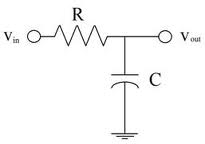
\includegraphics[scale=.75]{Rc_lowpass.png}
\caption{a diagram of a low pass filter}
\label{low-pass filter}
\end{figure}

\begin{figure}[H]
\center
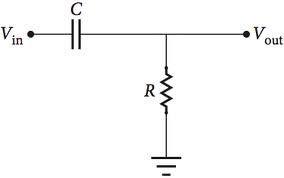
\includegraphics[scale=.6]{Rc_hipass.png}
\caption{a diagram of a high pass filter}
\label{high-pass filter}
\end{figure}

\subsection{LC filters}
Inductors are resistant to changes in current as seen in 
\begin{equation}
  \label{inductance voltage}
  V = L \frac{dI}{dt}
\end{equation}
where L is the inductance. when a current passes through, they store a
portion of the energy in their magnetic field. they behave like wire if
a current continuosly flows,  but once the current stops, the magnetic
field collapses, and so the energy stored goes into pushing electrons in
the direction they were flowing in. For a larger inductor, a larger
volatage is induced when the field collapses. The impedance of an
inductor is 
\begin{equation}
  \label{inductor impedance}
  Z_L = jwL
\end{equation}
For an RLC bandpass filter, it's purpose is to not allow a band 

\subsection{Diode}
A diode has nearly zero resistance to current flow in one direction and
bery high resistance in the other direction. Because of this, it serves
to convert alternating current into direct current, including modulation
(the varying a signal so that it may carry information in a waveform)
here namely an incoming fm signal so that the signal can be read. The
following is a table of data for a diode in series with a resistor,
which changed values for every set, and with a varying Voltage applied
across it.
\begin{table}[H]
\center
\begin{tabular}{|c|c|}
\hline
R = 56 $\Omega$ & $V_{in} = 1.2 V$ \\
\hline 
R = 150 $\Omega$ & $V_{in} = 1.2V$ \\
\hline
                   & $2V_{in} = 2.7V$ \\
\hline
                   & $3V_{in} = 4.7V$ \\
\hline
R = 1200 $\Omega$ & $V_{in} = 1.6V$ \\
\hline
                    & $2V_{in} = 3.1V$ \\
\hline
                    & $3V_{in} = 5V$ \\
\hline
R = 2700 $\Omega$ & $2V_{in} = 3.1V$ \\
\hline
                    & $3V_{in} = 4.7V$ \\
\hline
                    & $4V_{in} = 7.3V$ \\
\hline
R = 1200 $\Omega$ & $3V_{in} = 5V$ \\
\hline
                    & $4V_{in} = 7.2V$ \\
\hline
                    & $5V_{in} = 9.3V$ \\
\hline
\end{tabular}
\caption{Table showing the measured voltage across a diode with varying
  Voltages and resistances}
\label{tab.1}
\end{table}

\subsection{FM Demodulator}
Our finished FM receiver is presented in the following figure
\begin{figure}[H]
\center
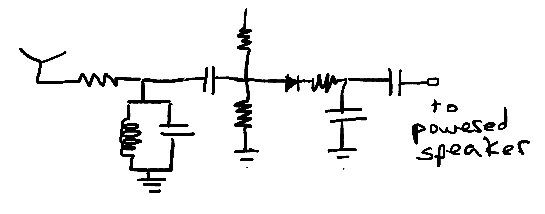
\includegraphics[scale=.5]{fm_demodulation.png}
\caption{An FM Demodulator, consisting of an antenna, an RLC circuit, a high pass
  filter, a diode, a low pass filter and a capacitor}
\label{FM Demodulator}
\end{figure}
In the FM Demodulator, The antenna acts acts as a tool to capture and
transmit radio signals to send down the circuit. When the current goes
into the RLC bandpass filter, there is a certain range of frequencies
that will be selected, from lab instructions, we had to use apprpriate
values for a change of frequency of 200 kHz given a 1 MHz sine wave, we
ended up calculating a resistance of 27 $\Omega$ using the equation
\begin{equation}
  \label{resistance for RLC}
  Q = w_{0}RC = \frac{f_{0}}{\Delta f_{3dB}}
\end{equation}
where we were given $f_0$ and $\Delta$ $f_{3dB}$ and we had to choose an
appropriate Capacitance, so due to a lack a capacitors, I chose 1
$\mu$F. To further simplify, I used $w_{0}$ = 2$\pi$$f_{0}$. And so that
is how we got our value for the resistor we'd be using. Next came the
high pass filter which served to filter out lower frequencies and only
allow the higher frequencies to get through after a bandpass had been
selected from the RLC, the cutoff point for which the -3dB point was
reached was defined to be 100 kHz. After this point, the band would have
to pass through the diode, which demodulated the incoming signal so that
the information (the music) could get through and to prevent any signal
from getting back thorugh. The signal was alternating but was changed to
direct current once it passed through the diode. From there there was a
low-pass filter in which its capacitor helped bring a continous signal
to the powered speaker. To elaborate more, the signal coming in was in
pieces, and as it got to the capacitor, it held charge, when another
sine wave of greater amplitude comes in,  then it held more energy, but
as soon as there is a sine wave of a lower amplitude relative to the
previous one before it,  the capcitor dissipates some of the energy and
when an even lower amplitude wave comes in, more energy is disspated,
this cycle continues so that a constant sine wave is created and can be
clearly heard through the speaker.

As for plots for this receiver, I did not do them, due to neglecting it
until some later time, which I then overestimated for the amount of time I
had left.


\section{Amplifiers, Week 2}

\subsection{Impedance mismatches in a transmission Line}
For a 15 meter cable, the pulse takes 2 that distance to make a round
trip from the source, through the cable, and back again to the source so 
\begin{equation}
  \label{pulse velocity}
  \frac{30 m}{750 ns} = 4\times10^{7} m/s
\end{equation}
The 750 ns came from observations of the oscilloscope of 3 divisions
multiplied by 250 ns per division thus giving us 750 ns travel
time. This speed of $4\times10^{7}$ m/s comes out to be a fraction of
the speed of light (2/15) 
When a resistor of 10 $\Omega$ was added, our square wave became
distorted; meaning that this 10 $\Omega$ resistor was not the proper one
to to terminate the the reflected wave, it seemed to be too small a
value because there was still a reflected wave coming back.
When instead a 56 $\Omega$ resistor was added, we got our original
square wave back, so the reflected wave was properly terminated. 

\subsection{Follower Circuit}
This circuit consists of a biased resistors acting as a voltage
divider. The emitter resistor is there for the purpose of measuring the
gain across the transistor. The gain in general is calculated as 
\begin{equation} 
  \label{gain equation} 
  g = \frac{Z_c}{Z_e}
\end{equation}
where the subscripts C and E refer to the collector and emitter
components respectively. Since for this follower the impedances are just
the two resistors, the gain is simply
\begin{equation}
  \label{gain resistor}
  g = \frac{R_c}{R_e}
\end{equation}

\subsection{Amplifier}
For the NPN BJT amplifier below
\begin{figure}[H]
\center
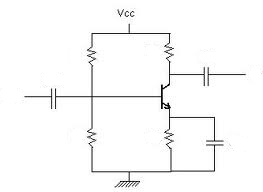
\includegraphics[scale=.6]{bjt_amplifier_lab2.png}
\caption{Our Amplifier Circuit}
\label{Amplifier}
\end{figure}
The way we measure gain is more complicated, since noe the emitter is no
longer attached to a resistor, but to a resistor and capacitor in
parallel. So now, $Z_c$ is represented by 
\begin{equation}
  \label{impedance for RC parallel}
  Z_c = \frac{1}{\sqrt{{\frac{1}{R^2} + w^2R^2}}}
\end{equation}
so now our gain can be calculated by \ref{gain equation}. So to get any
gain, all you would need to do, if you have known resistances, is simply
solve for the capacitance to get the gain you wanted. Also w = 2$\pi$f,
where f is the frequency given by the lab. So to calculate gain now,
then 
\begin{equation}
  \label{amplifier gain}
  g = \frac{1}{R_E\times\sqrt{{\frac{1}{R^2} + w^2R^2}}}
\end{equation}

\subsection{Speaker-Amplifier}
For our speaker amplifier, the receiver part has already been explained,
so after the signal has been demodulated by the diode and the signal
comes in as a continous sine wave it has to go through the amplifier
where it first meets a high pass filter (figure \ref{Amplifier}) to make
sure no lower frequencies will interfere, from there there the signal
enters the voltage divider, this is set a biasing point for the
trnsistor to work  in the range we want it to be in. The transistor is
used to isolate the two stages of the circuit. The emitter resistor
creates a voltage from the current passing through the emitter of the
transistor. If it wasn't there wouldn't be any voltage would go straight
to ground, preventing measurements. The Capacitors are there to stop DC
voltage from coming through and messing with the audio. 

The net effect of the amplifier is to take an incoming current and
amplify it. In our speaker-amplifier, we only measured a small
amplification of gain = 2 so our initial values for our resistors and
capacitors must have been wrong

If we attached a long cable between our amplifier and speaker, then we
should match the value of the impedance of the speaker 8 $\Omega$ and
the total impedance of the amplifier circuit, which totals to the sum of
the impedances of the emitter and collector as well as the resistances
of the voltage divider and the capacitor. If it matches this, then there
shouldn't be reflections that would otherwise create an echo.

\section{Week 3: Noise and the Central Limit Theorem}
\subsection{minicircuits amplifiers}
Unfortunately, with only one working amplifier supplied, our group
couldn't do any of the experiments rearding the amplifiers. Instead
there will just be a summary of some topics

\subsection{John-Nyquist Noise}
This is the thermal noise generated by the random motions of electrons
within a resistor, this current has a zero mean, but can vary. This
causes a fluctuating voltage across a resistor. The variance in the
voltage is 
\begin{equation}
  \label{variance}
  V^2 = 4k_BTBR
\end{equation}
where T is the Temperature of the resistor, and B is the bandwidth of the
frequency that will be measured.
By Ohm's law, the power of the signal generated by the resistor is 
\begin{equation}
  \label{power}
  P_{sig} = 4k_BTB
\end{equation}
Not all the power generated by a resistor can be passed through the
circuit, the only way in which the maximum amount of power can be
disspated is if the impedance of the load matches the resitor. 

\subsection{The Central Limit theorem}
In this theorem, if we consider a random sample size of size n, so that
the sequence of numbers are independently and identically distributed,
the mean of all samples will be normally distributed in 'a bell curve'.
From coding when we choose some maximum value for our distribution and
choose a sample size, and set some number of iterations (number of times
randomly chosen numbers go into a set sample size) we get a Normalized
distribution as shown by the following two graphs. 
\begin{figure}[H]
\center
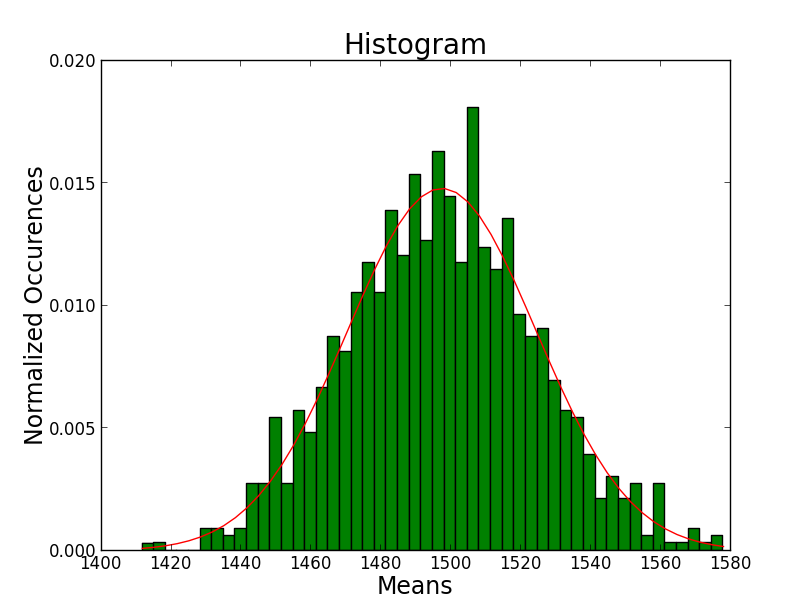
\includegraphics[scale=.6]{central_limit_3.png}
\caption{A normal distribution for 1000 iterations}
\label{central1}
\end{figure}
In this figure, I instructed my code to have sample sizes of 1000
numbers with numbers chosen randomly from a minimum value of 0 to
3000. After this, I chose for there to be 1000 samples (iterations) and
so when the means are plotted we see that there is a normalized curved
around 1500, which is the average of 0 to 3000. To show that the Central
limit theorem does in fact conform better when a larger amount of
iterations are made, I ran the same numbers but instead of 1000
iterations, I had it perform 1500 iterations so what we get now is 
\begin{figure}[H]
\center
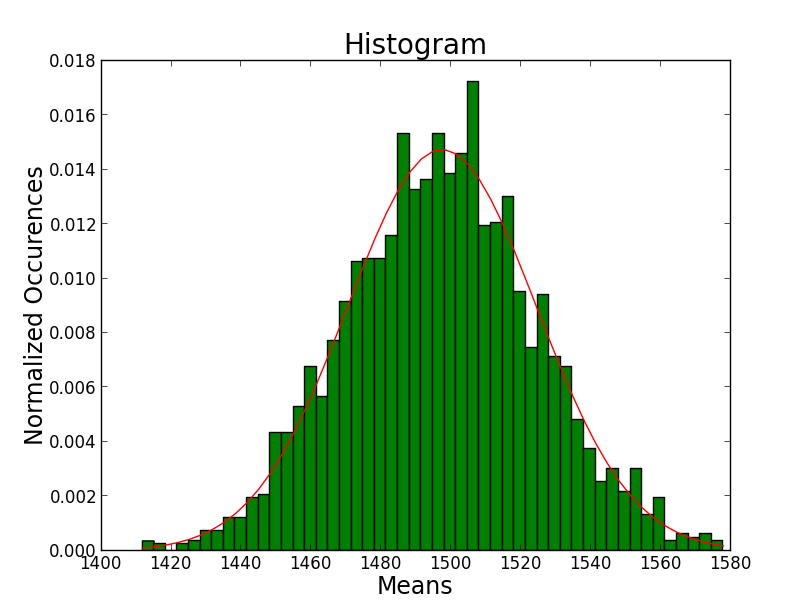
\includegraphics[scale=.6]{central_limit_4.png}
\caption{A normal distribution for 1500 iterations}
\label{central2}
\end{figure}
The diffrence in this graph compared to the previous graph is that we
see a greater conformity to a normalized distribution, with less
variance (as seen by the outliers not fitting under the gaussian curve), therefore, if I were to run this program again for 2000
iterations then my plot would reach a unit variance,  and have a 0 mean
around the value of 1500. 
As you increase the number of samples, N, then we would see that the
standard deviation would decrease by $\sqrt{N}$

\subsection{Amplifier Noise Results}
We could not measure any final noise due to the amplifiers being broken,
so there isn't even an estimate.

\section{Discussion}
In this lab I had problems, mainly with my own priorities, I would put
off the work for the week-ends and neglect plots for activities, which
hurt the results of the the main things we needed to include in the
report. Aside from that, the amplifier issue did prevent data collection
that would have been useful to analyze in future labs. As for results I
did manage to gain, there is a greater knowledge of how circuits work,
though not a thorough one, it was still enough to understand what each
configuration of circuit components can do. There is still a lack of
knowledge by my own fault. 


\section{Conclusion}
The results of these activities have proven useful for getting future
labs done in a shorter amount of time, at least if they are constructing
circuits from diagrams. These components acting as one will lead to an
easier undersdtanding of potentially more difficult circuits, like a
radio telescope, or at least understand the net effect on a signal by
some apparatus. For Radio astronomy in general, this practice with
circuits will at least help with trouble-shooting problems you could
potentially have; narrow the reasons why some thing may not be working.   

\end{document}